\chapter{Capítulo Aleatório}
\label{chap:CapAle}

Lista do capítulo da lista \ref{chap:CapAle}:

\begin{enumerate}
\item item a
\item item b
\item item c
	\begin{itemize}
	\item item d
	\item item e
	\item item f
		\begin{enumerate}[label*=\arabic*.]
		\item item g
		\item item h
		\item item i
			\begin{itemize}
			\item itemizeception
			\end{itemize}
		\end{enumerate}
	\end{itemize}
\end{enumerate}

CIRCUITÃO:

\begin{figure}[!htb] \label{fig:circuitevers}
\centering
\begin{tikzpicture}

\draw (0,0) to [sV] (0,2) to[closing switch] (2,2) to[lamp] (2,0) -- (0,0);
\draw (3,0)  to[R] (3,3);

\end{tikzpicture}
\caption{circuto massa}
\end{figure}

Juntando sem pular linha: 70~cm 
\hfill

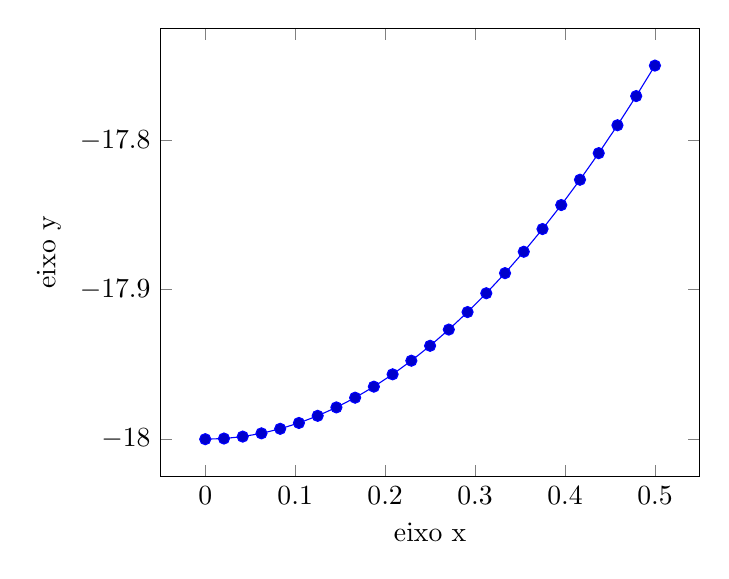
\begin{tikzpicture}
\centering
\begin{axis}[xlabel=eixo x,ylabel=eixo y]
\addplot+[domain=0:0.5]{x*x -18};
\end{axis}
\end{tikzpicture}